\documentclass[10pt]{sigplanconf}

%%% Packages %%%
\usepackage{caption}
\usepackage{color}
\usepackage{graphicx}
\usepackage{hyperref}
\usepackage{listings}
\usepackage{subcaption}
\usepackage{times}
\usepackage{url}
\usepackage{microtype}
%\usepackage{color,fullpage,microtype}
%\usepackage{graphicx,wrapfig,subfigure,titling}
%\usepackage{amssymb,amsmath,amssymb,amsfonts}
\usepackage{amsthm}
%\usepackage{textcomp}
%\usepackage{multirow}
%\usepackage{gensymb}
%\usepackage{array}
%\usepackage{times}
%\usepackage[sort]{cite}

%%% Author and Title %%%
\title{Immovable Objects Meet An Irresistible Force: \\
Meshing Memory Management for Compaction without Relocation}

\authorinfo{Emery D. Berger \and Andrew McGregor}{
  College of Information and Computer Sciences \\
  University of Massachusetts Amherst}{
  \texttt{emery@cs.umass.edu}, \texttt{mcgregor@cs.umass.edu}}

%%% Copyright Information %%%
\exclusivelicense
\conferenceinfo{OOPSLA'16}{XXX}
\copyrightyear{2016} 
\copyrightdata{XXX}
\doi{2815400.2815409}

%%% Set up microtype %%%
\microtypesetup{
  final,
  tracking=true,
  kerning=true,
  spacing=true,
  factor=1100,
  stretch=20,
  shrink=20
}
\SetTracking{encoding={*}, shape=sc}{0} % No tracking for smallcaps

%%% Caption formatting and spacing %%%
\captionsetup{font=small,labelfont=bf}
\setlength{\belowcaptionskip}{-5pt}
\setlength{\abovecaptionskip}{5pt}
\setlength{\floatsep}{5pt}

%%% Listings %%%
\definecolor{mygreen}{rgb}{0,0.6,0}
\definecolor{mygray}{rgb}{0.5,0.5,0.5}
\definecolor{mymauve}{rgb}{0.58,0,0.82}
\lstset{
  basicstyle=\footnotesize,        % the size of the fonts that are used for the code
  tabsize=2,                       % sets default tabsize to 2 spaces
  captionpos=none,                 % sets the caption-position to bottom
  keywordstyle=\color{blue},       % keyword style
  commentstyle=\color{mygreen},    % comment style
  stringstyle=\color{mymauve},     % string literal style
  keepspaces=true,                 % preserve spaces  
  morekeywords={*,...},            % if you want to add more keywords to the set
  numbers=left,                    % place line numbers on the left
  stepnumber=1,                    % step between line numbers
  numbersep=5pt,                   % how far the line-numbers are from the code
  numberstyle=\tiny\color{mygray}, % the style that is used for the line-numbers
  escapechar=\$                    % escape character for using latex commands in listings
}
\lstdefinelanguage{c++threads}[]{c++}{morekeywords={pthread_create,pthread_join,thread,join}}
\lstset{language=c++threads, basicstyle=\ttfamily\scriptsize,frame=trbl,tabsize=2}

%%% Custom Commands %%%
\newcommand{\mesh}{\textsc{Mesh}}
\newcommand{\punt}[1]{}

\newtheorem{definition}{Definition}
\newtheorem{theorem}{Theorem}[section]
\newtheorem{proposition}{Proposition}[section]
\newtheorem{corollary}{Corollary}[section]
\newtheorem{lemma}{Lemma}[section]
\newtheorem{conjecture}{Conjecture}[section]
\newtheorem{fact}{Fact}
\newtheorem{problem}{Problem}
\newtheorem{example}{Example}
\newtheorem{claim}{Claim}

\newcommand{\expec}[1]{\mathbb E\left [ #1 \right ]}
\newcommand{\rounddown}[1]{\left \lfloor  #1 \right \rfloor}
\newcommand{\roundup}[1]{\left \lceil  #1 \right \rceil}

%%% The Document %%%
\begin{document}

  \maketitle
  
\begin{abstract}
Because C and C++ objects cannot be relocated, memory allocators for
those languages cannot compact objects and thus can suffer potentially
catastrophic fragmentation. In a classic result, Robson showed that
such allocators can consume up to $(O \log M/m)$, where $M/m$ is the
ratio of the largest and smallest object request
sizes~\cite{robson1977worst}. We present a counterintuitive result: a
memory management algorithm that can perform compaction without
relocating objects. Our approach \emph{meshes} together objects from
separate pages whose virtual offsets do not overlap, compacting them
physically onto a single page while maintaining their virtual
addresses. Meshing depends on widely-available OS support and a
randomized algorithm that provides provably effective compaction with
high probability. We demonstrate that meshing is practical and
effective by implementing a prototype meshing memory allocator.
\end{abstract}

\section{Introduction}
\label{sec:introduction}

In unmanaged languages like C and C++ the memory addresses of objects
are directly exposed to the program, and as a result objects cannot be
relocated.  These languages let programmers store addresses in
integers, perform arithmetic on addresses, write them to and from
pipes, and convert integers into addresses.  Given such an adversarial
environment, a runtime system can not guarantee that it can identify
all object references at any given point in time.  Without precisely
identifying \textit{all} references objects can not safely be
relocated, as all locations that point to a moved object need to be
updated for the program to continue executing correctly.

Because objects can not be relocated, memory allocators for these
languages can not perform compaction and thus programs may suffer from
fragmentation.  Fragmentation is a result of the fact that while a
user's program manages memory at the granularity of \textit{bytes},
operating systems manage memory at the level of \textit{pages} (4 KiB
on most contemporary architectures).  Fragmentation occurs when a
small number of program objects require the reservation of a
corresponding large number of pages from the operating system.
Fragmentation can result in a program requiring orders of magnitude
more memory from the operating system than is required by the
semantics of the program.

Fragmentation is important because it exacerbates memory pressure --
one of the scarcest resources on modern computing devices.  70 percent
of Google Chrome crashes on low-RAM Android devices are caused by
Chrome running out of memory when attempting to display the
page~\cite{hara:whymemory}.  Embedded systems designed for the
Internet-of-Things (IoT), such as the Raspberry Pi Zero W, ship with
wireless networking, 3D graphics, and complete operating system stacks
but only hundreds of megabytes of memory~\cite{rpi:zero}.

Fragmentation has been widely
studied~\cite{johnstone:1998:fragmentation} and solved for managed
languages with \textit{moving
  compaction}~\cite{hansen:1969:compaction,fenichel:1969:compaction}
in the late 1960s.  Compaction minimizes fragmentation by moving live
objects close together.  Contemporary runtimes like the Hotspot
JVM~\cite{microystems2006memory}, The .NET
VM~\cite{microsoft:dotnet-gc}, the SpiderMonkey JavaScript
VM~\cite{mozilla:spidermonkey-compaction} and others implement moving
compaction as part of their garbage collection algorithms.

We present \Mesh, the first runtime system to bring precise compaction
to unmanaged languages like C and C++.  \Mesh uses randomization to
provably bound the impact of fragmentation with high probability.

\subsection{Contributions}
\label{sec:contributions}

This paper makes the following contributions:

\begin{itemize}
\item It introduces the concept of \textbf{meshing}, a mechanism that
  provides \textit{compaction without relocation} for unmanaged
  languages.  Meshing eliminates memory fragmentation in languages
  like C and C++ with high probability, and we identify analytic
  bounds on the savings possible and achievable.
\item It presents \textbf{\Mesh}, a runtime system and memory
  allocator that delivers compaction without relocation for binaries
  compiled from unmanaged languages like C, C++ and Rust.  We evaluate
  \Mesh's performance empirically and analytically.
  % TODO: mention evaluation results
\end{itemize}

The rest of this paper is organized as follows.
Section~\ref{sec:meshing} introduces the concept of meshing and show
how our approach reduces fragmentation in a representative unmanaged
program.  Section~\ref{sec:allocator} details \Mesh's efficient memory
allocator.  Section~\ref{sec:theory} presents the theoretical results
that make meshing efficient and
practical. Section~\ref{sec:evaluation} provides an empirical
evaluation of \Mesh, and section~\ref{sec:discussion} discusses how
several classes of applications would benefit from deeper integration
with \Mesh.  Finally, section~\ref{sec:related-work} discusses related
work, and section~\ref{sec:conclusion} concludes this paper.

%\section{Overview}
\label{sec:meshing}

\begin{figure}[!t]
\centering
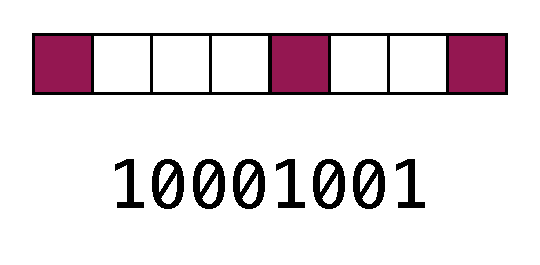
\includegraphics[width=.3\textwidth]{figures/bitmap_bitstring}
\caption{The bitmaps managing the allocated space in a span
  (visualized as allocated objects in the span, top) can be
  represented as bitstrings of 0s and 1s (bottom), where a 1
  corresponds to an allocated object and 0 to free space.}
\label{fig:bitmap-bitstring}
\end{figure}

Meshing is the problem and process of minimizing physical memory use
(measured as resident-set size, or RSS) without modifying allocated
virtual addresses.

A \textit{span} is a contiguous region of memory, and the size of a
span is a multiple of the page size between 4 KiB and 128 KiB.  Each
span allocates objects of a single-size only, for example a 4 KiB span
might hold 32 objects of size 128 bytes.  We can represent a span by a
\textit{bitstring}, a string with a 1 for an allocated object at that
offset from the start of the span and 0 otherwise.  The length of the
bitstring is the number of objects that span holds.

We say $t$ spans \textit{mesh} iff the logical-AND of their bitstrings
($s_i$) of length $t$ is zero. INCORRECT? THIS LETS US MESH TWO 11111 STRINGS WITH ONE 00000 STRING FOR INSTANCE. Formally:

\begin{align}
  \forall k \in [0, b-1]. \sum_{0 \leq i \leq t} s_i[k] \leq 1
\end{align}

This definition characterizes the constraints of the technique by which 
meshing is possible, wherein two or more spans are meshed or "stacked" 
on top of each other.  Each object in the resulting meshed span resides at the same 
offset as it did in its original span, as in Figure 2.  This is only possible when no two spans
have objects at the same offset.  After this process all objects reside
in a single span, and all other spans are empty and can be used anew
for allocation.

The layout and management of a program's heap guide how we consider
meshing.  In a running program, the heap is managed as a number of
different \textit{size classes} along with a region consisting of
large allocations.  Allocations are fulfilled from the smallest size
class they fit in (e.g. an allocation request for 50 bytes is
satisfied by the 64-byte size class), and objects larger than 16 KiB
are individually served from the large allocation region.

We treat each size class as an independent instance of the meshing
problem, and large allocations are not meshed.  As large allocations
are all many multiples of the page size significant fragmentation
between them does not exist.  The number of size-classes is fixed at
compilation time and constant during the execution of a program.

From here, we consider meshing as dealing with a single size-class,
and refer to all spans within this size class as $S$.  If we want to
mesh the entire heap, this means solving $n$ instances of the meshing
problem, where $n$ is the number of size classes.


\begin{figure}[!t]
  \centering
  \begin{subfigure}[t]{.5\textwidth}
    \centering
    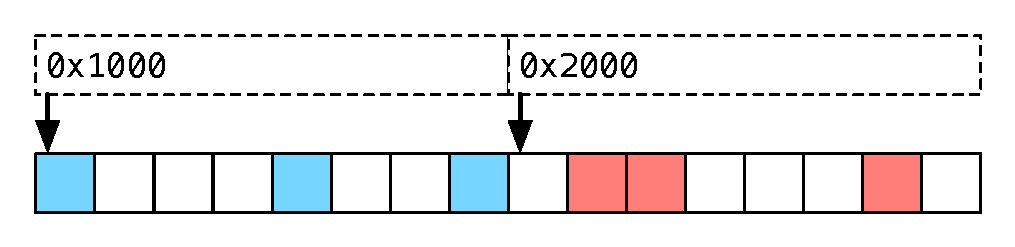
\includegraphics[width=\textwidth]{figures/before_meshing}
    \caption{Two adjacent spans that are candidates for meshing.}
  \end{subfigure}%
  ~

  \begin{subfigure}[t]{.5\textwidth}
    \centering
    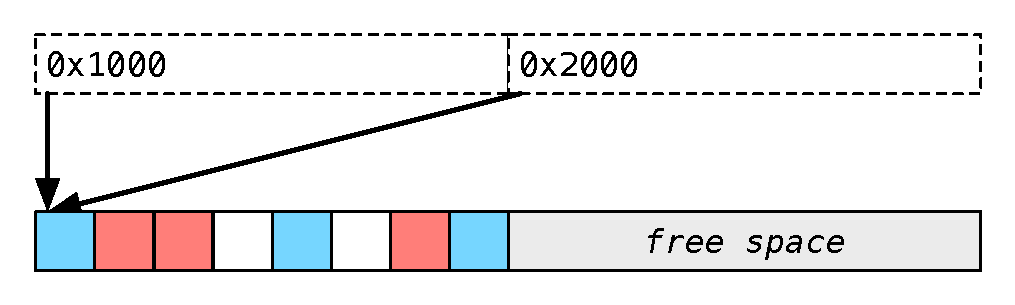
\includegraphics[width=\textwidth]{figures/after_meshing}
    \caption{After meshing, both virtual spans refer to the same
      physical \newline span, with live objects interleaved.}
  \end{subfigure}
  \caption{Virtual and physical memory layout before and after
    meshing.  After meshing, physical span occupancy has increased
    from 37.5\% to 75\% and one physical span has been returned to the
    OS for reuse.}
  \label{fig:meshing}
\end{figure}

Finally, meshing relies on the fact that there are two types of spans,
virtual and physical.  A \textit{virtual} span refers to the memory
addresses visible to the program being executed, while a
\textit{physical} span corresponds to the area in memory where
allocated objects live.  Meshing is concerned with minimizing the
count of in-use physical spans without modifying or moving virtual
spans.  As noted in Section~\ref{sec:introduction}, we cannot change
or modify virtual addresses returned from the allocator, as we do
not have a way to enumerate and update all references the program has
stored.  Since the last two digits of a virtual address directly specify the offset of the referenced object in the span, objects cannot
be safely relocated to a different offset, leading to our 

Allocated objects and free space within a span are tracked by the
memory allocator as a bitmap (see Section~\ref{sec:allocator}) -- the
in-memory representation of a bitstring.  For example, for objects of
size 32 and a span size of 4 KiB, the span can hold 128 32-byte
objects, so allocated objects are be tracked with a 128-bit bitmap.
Each allocated object in a running program has a unique
\textit{(bitmap, offset)} tuple.  Bitmaps are between 8 and 256-bits
in length.

We can therefore think of the meshing problem as that of partitioning
a set of equal-length bitstrings such that the bitstrings in each subset
mesh.  An optimal partition would minimize the number of such subsets.
This abstraction allows us to analyze the complexity of this computational
task in Section~\ref{sec:theory}.
\section{Analysis}
\label{sec:analysis}

Pick $m$ random strings of length $b$ with $n$ ones.
Let $X^s$ be the number of copies of string $s$ and note that $X^s \sim Bin(m,p)$ where $p=1/{b \choose n}$. 
We say a pair of strings $s^1$ and $s^2$ are combinable if $s^1\cdot s^2=0$. A set of strings is combinable if they are pairwise combinable.

\subsection{Combining Pairs of Strings}

Partition the set of all binary strings of length $b$ with $n$ ones into the sets
\[A=\{x\in \{0,1\}^b: |x|=n, x_1=1\}\] and \[
B=\{x\in \{0,1\}^b: |x|=n, x_1=0\} \ .\]


%Consider pairing combinable strings greedily. 
In the case where $n=b/2$, the number of unpaired strings is 

\[U=\sum_{s\in A} |X^s-X^{\bar{s}}|\] 
since $s$ is only combinable with its complement $\bar{s}$ when $n=b/2$.

\begin{theorem}
\[D_m(p)/(2p) \leq E(U) \leq D_m(p)/p \ ,\]
where 
\[D_m(p)=2(1-p)^{N-\rounddown{mp}}p^{1+\rounddown{mp}}(\rounddown{mp}+1){N\choose \rounddown{mp}+1}\]
and note that $\sqrt{mp(1-p)}/\sqrt{2} \leq D_m(p)\leq \sqrt{mp(1-p)}$ on the assumption that $1/m\leq p\leq 1-1/m$.
\end{theorem}
\begin{proof}
Let $X\sim Bin(m,p)$.
By the triangle inequality and linearity of expectation:
\[E[U]=\sum_{s\in A} E[|X^s-X^{\bar{s}}|]\]
\[\leq \sum_{s\in A} E[|X^s-mp|] + E[|X^{\bar{s}}-mp|]\]
\[=1/p \cdot E[|X-mp|]\]

Define the event,
\[A=\{X^s\geq mp\geq X^{\bar{s}} \mbox{ or } X^s\leq mp\leq  X^{\bar{s}}\}\]
By linearity of expectation:
\begin{eqnarray*}
E[U]
& \geq & 
\sum_{s\in A} P(A) 
E[|X^s-X^{\bar{s}}| \big | A] \\
& \geq & 1/2 \cdot 
\sum_{s\in A} E[|X^s-mp|] + E[|X^{\bar{s}}-mp|]\\
& = & 1/(2p)  E[|X-mp|]
\end{eqnarray*}

The result follows since by a theorem of De Moivre, the absolute deviation of the binomial distribution is 
\[E[|X-mp|]=D_m(p)\]
\[=2(1-p)^{m-\rounddown{mp}}p^{1+\rounddown{mp}}(\rounddown{mp}+1){N\choose \rounddown{mp}+1}\] 
The bound on $D_m(p)$ is due to Blyth (1980) and  Berend and  Kontorovich (2013).
\end{proof}

\begin{corollary}
For any $n\leq b/2$, \[\lim_{m\rightarrow \infty} E(U)/m=0\] i.e.,  the fraction of strings that are unpaired tends to zero when $m\rightarrow \infty$.
\end{corollary}
\begin{proof}
By the previous theorem, if $n=b/2$, $E(U)/m \leq D_m(p)/(mp)\leq \frac{\sqrt{(1-p)}}{\sqrt{mp}} \rightarrow 0$ as $m\rightarrow \infty$. Note that the bound also holds for $n\leq b/2$ because decreasing the weight of the strings only increases the probability that a pair of strings is combinable.
\end{proof}

\subsubsection{Random Graph Approach}
Consider the graph where nodes correspond to sampled strings where there
is an edge between two nodes iff the strings are compatible. So each
edge is present with probability $q={b-n \choose n}/{b\choose
  n}$. Note that edges are pair-wise independent but not three-wise
independent (e.g., there are fewer triangles than you would
expect). However, the number of incident edges on a node is
$Bin(m-1,q)$.

Let $M$ be the size of the maximum in the graph. This number is the maximum
number of mutually combinable pairs. Had the edges been fully
independent then $E[M]\geq \frac{m}{2}\frac{c}{c+1}$ if $c=q(m-1)/2$
is constant.

Assuming $mq$ is a small constant less than 1, the following lemma gives a good bound.
\begin{lemma}
\begin{eqnarray*}
& & \frac{m}{2} \cdot  \max \left (2-2(1-q)^{m-1}-(m-1) q, \right . \\
& & \left . (m-1) q\left (1-2q+\frac{{b-2n \choose n}}{{b \choose n}}\right )^{m-2}\right ) \\
&\leq & E(M) \\
& \leq & \frac{m}{2} \cdot  \min(1,(m-1)q) \ .
\end{eqnarray*} 
E.g., for $b=32, n=14$ and $m=5000$ we get $78.5 \leq E(M)\leq 81$. 

Since $E(M)$ is monotonically increasing in $q$, it follows that for $q\geq 1-2^{-1/(m-2)}$ we may deduce that, 
\[0.307 \times \frac{m}{2}=(1-\ln(2))\frac{m}{2} \leq E(M)\]
since $2-2(1-q)^{m-1}-(m-1) q$ is maximized at $q=1-2^{-1/(m-2)}$.
%
%(1-q)^(m-2)=1/2
%(m-2) lg (1-q)=-1
%q=1-2^(-1/(m-2))
%Note that the lower bounds are not increasing in $q$ for all values of $q$ but we can always maximize over smaller values of $q$.
%$(m-1) q (1-2(m-2)q)$ is maximized at $mq\approx 1/4$ and at that point takes the value $1/8$. Hence, as soon as $mq\geq 1/4$ we expect to get a matching whose size is at least an eight as large as the maximum possible matching.

It also follows from the upper bound,
\[P(M\geq 1)\leq {m \choose 2} q \ .\]
E.g., for $b=32, n=14$, we need $m\geq 394$ for $P(M\geq 1)\geq 1/2$.
\end{lemma}

\begin{proof}
The upper bound follows from the fact that $M$ is at most the number
of edges in the graph. Hence, $E(M)\leq {m \choose 2} q$.

Let $I$ be the number of \emph{isolated edges}; an edge $uv$ is
isolated if $uv$ is the only edge in the graph incident on $u$ or
$v$. Let $I_e=1$ if $e$ is isolated, and $I_e=0$ otherwise. Then
\begin{eqnarray*}
& & E(I_{uv}) \\
&=& P(uv\in G)P(uw, vw \not \in G ~ \forall w\in V\setminus \{u,v\}| uv\in G)\\
& =& q\left (1-2q+\frac{{b-2n \choose n}}{{b \choose n}}\right )^{m-2} \ .
\end{eqnarray*}
The first lower bound then follows from $E(I)=\sum_e E(I_e)$.

Another lower bound follows from the following idea. Consider the
graph formed by removing all but one incident edge from any node with
two or more incident edges. The remaining graph is a matching. The
expected size of this matching is at least (because some edge removals
may have been counted twice):

\begin{eqnarray*}
& & {m \choose 2} q-\sum_v E(\max(deg(v)-1,0) \\
&=&
{m \choose 2} q
-m\sum_{d=1}^{m-1} {m-1\choose i} q^i (1-q)^{m-1-i}(i-1)\\
&=& {m \choose 2} q-m[(m-1)q-1+(1-q)^{m-1}]\\
&=& m(1-(1-q)^{m-1})-{m \choose 2} q \ .
\end{eqnarray*}
\end{proof}

Note that the expected number of triangles in such a graph is ${m
  \choose 3} {b-n \choose n}/{b\choose n} {b-2n \choose n}/{b\choose
  n}$. For example, if $b=32, n=10, m=1000$, we expect less than two
triangles. Hence, with such parameters, it only makes sense to look for
pairs of blocks that can be combined rather than sets of three or more
blocks that can be combined together.

%Another bound:
%\[E(M) \geq \frac{m}{2} (m-1)q/2
\subsubsection{Random Walk Approach}

Keep on adding strings up to $m$. If a new string combines with an
existing one, remove both. Let $S_t$ be number of strings at time
$t$. Let $q={b-n \choose n}/{b\choose n}=(1-n/b)(1-n/(b-1))\ldots
(1-n/(b-n+1))\geq (1-n^2/(b-n+1))$. Then,

\[P(S_{t+1}=S_t-1)\geq q\]
\[P(S_{t+1}=S_t+1)\leq 1-q\]

If $q\leq 1/2$ then $E[S_t]=O(\sqrt{t})$ and $q\leq 1/2$ if $b\geq
2n^2+n-1$. As a consequence, if $q\leq 1/2$,  we expect the number of
unpaired strings to go to zero.
%\[P(S_{t+1}=S_t-1)\geq 1-(1-q)^{S_t}\geq 1-e^{-S_t q}\]
%\[P(S_{t+1}=S_t+1)\leq (1-q)^{S_t}\]
%\[
%2(1-p)^{N-\rounddown{Np}}p^{\rounddown{Np}}(\rounddown{Np}+1){N\choose \rounddown{Np}+1}
%\leq 
%\]

\subsection{Combining Multiple Strings}
Note that this is only possible if $n\leq b/3$.

\begin{lemma}
Define a graph $G$ where each string corresponds to a node and there
is an edge between two nodes if the two strings are \emph{not}
combinable. Then, the optimal number of combined strings is the
chromatic number of $G$.
%The number of combined strings 
\end{lemma}

Unfortunately, the edges of $G$ are not independent. Had they been
independent, we would have been able to appeal to existing analysis to
show that the expected value of the chromatic number is
\[
\frac{m}{2\log_{1/q} m}\approx \frac{(1-q)m}{2 \ln m}
\]
where $q$ is the probability of being combinable. 

The dependencies between edges means $(u,v)$ and $(v,w)$ present
implies $(u,w)$ are less likely to be present.

However, the following lemma gives a weaker bound for our case:
\begin{lemma}
It is possible to combine strings such that less than $(1+\epsilon)
(m-1)(1-q)+1$ remain with probability at least $1-me^{-\epsilon^2
  (m-1)(1-q)/3}$. For example, if $b=10, n=2, m=10000$, then the final
number of strings is at most $4156$ with probability at least
$1-3.92030 \times 10^{-13}$ by setting $\epsilon=0.1$.
\end{lemma}

\begin{proof}
The result follows because a greedy algorithm can color a graph in
$\Delta+1$ colors where $\Delta$ is the maximum degree of the graph.
Pick an arbitrary node $v$ and let the degree of $v$ be $D$. Then
$E[D]=(m-1)(1-q)$ and by the Chernoff bound
\[P(D\geq (1+\epsilon) (m-1)(1-q)] \leq e^{-\epsilon^2 (m-1)(1-q)/3}
 \ .\]

Hence by the union bound, the probability that all degrees at less
than $(1+\epsilon) (m-1)(1-q)$ is at most $me^{-\epsilon^2
  (m-1)(1-q)/3}$.

\end{proof}

%\input{implementation}
%\section{Evaluation}
\label{sec:evaluation}

We evaluate \Mesh in three ways.  We show that under an adversarial
program, \Mesh is able to recover from fragmentation much better than
other allocators.  As a case-study, we run Firefox under \Mesh and
identify that \Mesh may be able to recover ~10\% of overall memory
using \Mesh.  Finally, we run several benchmarks from the SPEC 2006
benchmark suite and show that \Mesh performs efficiently.

\subsection{High-fragmentation Performance}

Fragmentation happens when a sparse number of small objects requires
many pages of memory from the operating system, and we test \Mesh
under an adversarial program that attempts to achieve high
fragmentation.

Our adversarial program works as follows: It allocates 128 MiB of
512-byte objects, and then it frees every other object.  Next, it
allocates 64 MiB of 1024-byte objects, and frees every other object.
At the end of the program, the object has references to 128 MiB of
`live' allocations.  This program forces fragmentation, as there is no
consecutive space available after freeing every other allocation to
satisfy any new allocation.

When run under both TCMalloc and GNU libc's default malloc, the
application has a resident-set size of over 255 MiB, a memory blowup
of almost 2x due entirely to fragmentation.

When run under \Mesh where \Mesh is explicitly asked to mesh at the
end of the allocation cycle, memory usage drops to under 155 MiB, only
1.2x more than the application is referencing and a relative savings
of 100 MiB.

\subsection{Firefox}

Firefox is a web browser, a modern dynamic application that uses
between hundreds of megabytes and gigabytes of memory under standard
usage.  Firefox includes a Just-in-time compiler for JavaScript, and
manages memory for JavaScript objects on its own, in an isolated,
compacting, garbage collected heap.  Firefox does use the system (or a
bundled) allocator for significant portions of its allocated memory,
especially the Document Object Model and non-JS objects.

We run Firefox under \Mesh and are able to write the internal state of
\Mesh's data structures (such as the MiniHeap bitmap) to disk.  We
analyze these and show that the potential memory savings from being
able to mesh near-optimally is a reduction of 25\% the amount of
memory used for small objects (the objects we manage with MiniHeaps
and store in a meshable region of memory), which could translate to
~10\% overall reduction in memory usage for Firefox.

%% Additionally, we are able to show the occupancy of spans across
%% different size classes, as seen in Figure~\ref{fig:ff-occupancy}.
%% This data was reported after opening Firefox, navigating to Amazon,
%% and scrolling to the bottom of the page.  Intuitively, as the string
%% length increases (for smaller size classes), average occupancy
%% decreases.

\section{Related Work}
\label{sec:related}

BiBoP allocators.

\paragraph{Randomized memory management.} Several previous memory managers have employed randomization,
primarily for fault tolerance and
security~\cite{Novark:2010:DSH:1866307.1866371, 1134000, 1346296,
  1250736}. DieHard uses randomized memory allocation to provide
\emph{probabilistic memory safety}, which enables (probabilistically)
correct execution in the face of memory usage errors like heap buffer
overflows and use-after-free~\cite{1134000}. Archipelago extends
DieHard by placing each object in a randomly-selected page in a 64-bit
address space, significantly extending its ability to tolerate memory
errors~\cite{1346296}. Archipelago reduces its footprint by copying
unused objects into a conventional heap and discards the backing
physical page; it then uses virtual memory page protection to
intercept reads and re-instantiates the physical page on
demand. DieHarder extends DieHard to provide security against attacks
that exploit memory errors~\cite{Novark:2010:DSH:1866307.1866371},
while Exterminator leverages a randomized memory allocator to perform
statistical inference and automatically fix the application by
generating ``runtime patches''~\cite{1250736}. Stabilizer randomizes
the placement of code, stack frames, and heap objects to enable
statistically sound performance evaluation~\cite{stabilizer:asplos13};
we adopt Stabilizer's shuffling heap approach. Unlike all of these,
meshing uses randomization to enable it to effectively compact objects.

\paragraph{Virtual memory approaches.}
Appel and Li outline a number of approaches for using virtual memory
in user programs~\cite{Appel:1991:VMP:106972.106984}. Numerous memory
managers have exploited virtual memory primitives for a variety of
purposes~\cite{Novark:2010:DSH:1866307.1866371,1346296,Appel:1988:RCC:53990.53992,Boehm:1991:MPG:113445.113459,Dhurjati:2006:EDD:1135532.1135707,electricfence}. The
only memory manager that merges virtual pages is Hound, a memory leak
and ``bloat'' detector~\cite{1542521}. Hound uses periodic page
protection to track accesses and thus identify stale objects. By
allocating objects sequentially so they are age-segregated, it
eventually isolates leaked objects and bloat on their own pages. To
avoid mixing young and old objects, Hound does not reuse freed slots
on a page until it becomes completely empty. Because this lack of
reuse could lead to catastrophic memory consumption, Hound merges
virtual pages onto physical pages as a backstop. Meshing adapts this
approach and combines it with a randomized algorithm that lets it
effectively merge pages regardless of allocation pattern. Unlike
meshing, Hound's deterministic allocation strategy cannot guarantee
successful compaction and is best-effort only.

%\section{Conclusion}
\label{sec:conclusion}

This paper introduced \textbf{meshing}, a novel mechanism that
provides \textit{compaction without relocation} for unmanaged
languages.  Meshing eliminates memory fragmentation in languages like
C and C++ with high probability.

We think meshing is applicable both to unmanaged languages like C and
C++, but also potentially interesting for managed language runtimes
that don't have a clear path to supporting compaction, such as Go's
garbage collector.

  
%  \newpage
  
\bibliographystyle{abbrv}
\bibliography{mesh,emery}

\end{document}
